
% v2-acmsmall-sample.tex, dated March 6 2012
% This is a sample file for ACM small trim journals
%
% Compilation using 'acmsmall.cls' - version 1.3 (March 2012), Aptara Inc.
% (c) 2010 Association for Computing Machinery (ACM)
%
% Questions/Suggestions/Feedback should be addressed to => "acmtexsupport@aptaracorp.com".
% Users can also go through the FAQs available on the journal's submission webpage.
%
% Steps to compile: latex, bibtex, latex latex
%
% For tracking purposes => this is v1.3 - March 2012
\documentclass[prodmode,acmtecs]{acmsmall} % Aptara syntax
\usepackage[spanish,polish]{babel}
\usepackage[T1]{fontenc}
\usepackage{fancyvrb}
\usepackage{graphicx,hyperref}
\newcommand\cutout[1]{}


\usepackage[table]{xcolor}
\usepackage[utf8]{inputenc}
\usepackage[parfill]{parskip}
\usepackage{tabulary}
\PassOptionsToPackage{hyphens}{url}
\usepackage{hyperref}    
\usepackage[capitalize]{cleveref}


% Metadata Information
% !!! TODO: SET THESE VALUES !!!
\acmVolume{0}
\acmNumber{0}
\acmArticle{CFP}
\acmYear{0}
\acmMonth{0}

\newcounter{colstart}
\setcounter{page}{4}

\RecustomVerbatimCommand{\VerbatimInput}{VerbatimInput}%
{
%fontsize=\footnotesize,
fontfamily=\rmdefault
}


\newcommand{\UnderscoreCommands}{%\do\verbatiminput%
\do\citeNP \do\citeA \do\citeANP \do\citeN \do\shortcite%
\do\shortciteNP \do\shortciteA \do\shortciteANP \do\shortciteN%
\do\citeyear \do\citeyearNP%
}

\usepackage[strings]{underscore}



% Document starts
\begin{document}


\setcounter{colstart}{\thepage}

\acmArticle{CFP}
\title{{\huge\sc SIGLOG Monthly 261}

 May 2025}\author{ELLI ANASTASIADI\affil{Aalborg University, SE}\vspace*{-2.6cm}\begin{flushright}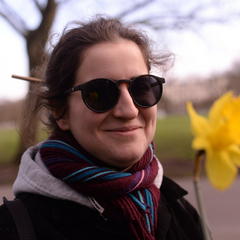
\includegraphics[width=30mm]{elli_anastasiadi.png}\end{flushright}}\begin{abstract}May 2025 edition of SIGLOG Monthly, featuring deadlines, calls and community announcements.
\end{abstract}


\maketitlee

\href{https://lics.siglog.org/newsletters/}{Past Issues}
 - 
\href{https://lics.siglog.org/newsletters/inst.html}{How to submit an announcement}
\section{Table of Contents}\begin{itemize}\item DEADLINES (\cref{deadlines}) 
 
\item SIGLOG MATTERS 
 
\begin{itemize}\item LICS 2025 (\cref{LICS2025})
\item LMW@LICS25 (\cref{LMWLICS25})
\end{itemize} 
\item CALLS 
 
\begin{itemize}\item GandALF 2025 (CALL FOR PAPERS) (\cref{GandALF2025})
\item Express/SOS 2025 (CALL FOR PAPERS) (\cref{ExpressSOS2025})
\item PODS 2026 (CALL FOR PAPERS) (\cref{PODS2026})
\item FROM 2025 (CALL FOR PAPERS) (\cref{FROM2025})
\item BMQL 2025 (CALL FOR PAPERS) (\cref{BMQL2025})
\item FAST TRACK ICLP 2025 (CALL FOR PAPERS) (\cref{FASTTRACKICLP2025})
\item FM 2026 (CALL FOR PAPERS) (\cref{FM2026})
\item DisCoTec 2025 (CALL FOR PARTICIPATION) (\cref{DisCoTec2025})
\item BLC 2025 (CALL FOR PARTICIPATION) (\cref{BLC2025})
\item ACKERMANN AWARD 2025 (CALL FOR NOMINATIONS) (\cref{ACKERMANNAWARD2025})
\item FSCD 2027 (CALL FOR LOCATION) (\cref{FSCD2027})
\end{itemize} 
\end{itemize}\section{Deadlines}\label{deadlines}\rowcolors{1}{white}{gray!25}\begin{tabulary}{\linewidth}{LL}LFMTP 2025:  & May 02, 2025 (Abstract deadline), May 09, 2025 (Paper deadline) \\
LSFA 2025:  & May 05, 2025 (Abstract), May 12, 2025 (Paper) \\
LOPSTR 2025:  & May 09, 2025 (Abstract), May 16, 2025 (Paper) \\
LMW@LICS25:  & May 10, 2025 (Travel support application) \\
DisCoTec 2025:  & May 23, 2025 (Early registration), Jun 11, 2025 (Late registration) \\
EuroProofNet Symposium 2025:  & May 25, 2025 (deadline for talk proposals and funding requests) \\
iFM 2025:  & May 30, 2025 (Abstract Submission), Jun 06, 2025 (Paper Submission), Aug 15, 2025 (Artifact Registration), Aug 01, 2025 (Artifact Submission 22) \\
GandALF 2025:  & May 30, 2025 (Paper  deadline) \\
DC 2025:  & Jun 01, 2025 (Paper) \\
DaLi 2025:  & Jun 01, 2025 (Abstract deadline), Jun 05, 2025 (Full paper deadline) \\
Express/SOS 2025:  & Jun 03, 2025 (Paper) \\
PODS 2026:  & Jun 03, 2025 (Abstracts), Jun 10, 2025 (Full papers) \\
BMQL 2025:  & Jun 10, 2025 (Submission) \\
FAST TRACK ICLP 2025:  & Jun 15, 2025 (IJCAI FAST TRACK Papers), May 15, 2025 (Abstracts or RECENTLY PUBLISHED track) \\
ACKERMANN AWARD 2025:  & Jul 01, 2025 (nominee s) \\
FM 2026:  & Nov 25, 2025 (Abstract Submission), Dec 02, 2025 (Full Paper Submission) \\
\end{tabulary}
\section{LICS 2025: Fortieth Annual ACM/IEEE Symposium on LOGIC IN COMPUTER SCIENCE (LICS)}\label{LICS2025}  23–26 June 2025\\ 
  \href{https://lics.siglog.org/lics25/}{https://lics.siglog.org/lics25/}\\ 
CALL FOR PARTICIPATION 

\begin{itemize}\item  Registration: \href{https://register.comp.nus.edu.sg/LICS2025/}{https://register.comp.nus.edu.sg/LICS2025/} 
 
\item  Local information: \href{https://lics.siglog.org/lics25/local.php}{https://lics.siglog.org/lics25/local.php} 
 
\item  Invited talks and tutorials from Anuj Dawar, Rustan Leino, Christine Tasson, Hongseok Yang 
 
\item  List of accepted papers: \href{https://lics.siglog.org/lics25/accepted.php}{https://lics.siglog.org/lics25/accepted.php} 
 
\end{itemize}\section{LMW@LICS25: 13th Logic Mentoring Workshop}\label{LMWLICS25}  \href{https://logic-mentoring-workshop.github.io/lics25/}{https://logic-mentoring-workshop.github.io/lics25/}\\ 
  23 June 2025, Singapore\\ 
  co-located with Logic in Computer Science (LICS) 2025\\ 
CALL FOR PARTICIPATION 

\begin{itemize}\item  Students can apply to have their expenses covered by the Logic Mentoring Workshop Travel Support (see below).  
 
\item  Attending a conference such as LICS can be a transformative experience. It exposes participants to cutting-edge research and can open up new research avenues and collaboration opportunities. The Logic Mentoring Workshop introduces young researchers to the technical and practical aspects of a career in logic research. It is targeted at students, from senior undergraduates to doctoral students, and will include tutorials and plenary talks as well as a panel discussion, where experienced researchers from the field answer career-related questions from the audience. 
 
\item  The workshop will be an on-site event, co-located with the Logic in Computer Science conference (LICS’25, \href{https://lics.siglog.org/}{https://lics.siglog.org/}) one of the most prestigious conferences on the topic.  
 
\item  REGISTRATION and PROGRAM 
 
  Registration is set up through the LICS website. The cost of the workshop is included in the registration for LICS, and separately costs 80 SGD. The detailed program will be announced at \href{https://logic-mentoring-workshop.github.io/lics25/}{https://logic-mentoring-workshop.github.io/lics25/} closer to the workshop.  
 
\item  TRAVEL SUPPORT 
 
  Students (undergrad, master's, and PhD alike) can apply to have their costs (some or all) covered by our sponsors, the National Science Foundation (NSF) and Jane Street.  
 
Travel support application: May 10th (applications are accepted after that date if funds allow) 
 
  Apply by filling this form: \href{https://docs.google.com/forms/d/1won7RTFgMbMtzhNiAARP5BzXTLPJKVcAj9zyIlmqVL8}{https://docs.google.com/forms/d/1won7RTFgMbMtzhNiAARP5BzXTLPJKVcAj9zyIlmqVL8} 
 
\item  LICS BUDDY 
 
  Is this the first conference you will attend in person? We have all been there. You might not feel comfortable if you don't know anyone. Join our Buddy Program, and we will help you to get in touch with another mentoring workshop attendee. Every newcomer will be assigned either a more experienced peer or another newcomer, so you are not alone. For those who are not attending a conference for the first time, being a buddy is a way for you to help the community to grow and introduce less experienced students to the field. If you are interested, write an email to lschuetze@mpi-sws.org 
 
\item  ORGANIZING COMMITTEE 
 
  Elli Anastasiadi, Linus Richter, Lia Schütze, Chana Weil-Kennedy 
 
\end{itemize}\section{GandALF 2025: 16th International Symposium on Games, Automata, Logics, and Formal Verification}\label{GandALF2025}  Valletta, Malta, 15-18 September 2025.\\ 
  \href{https://gandalfsymposium.github.io/2025/}{https://gandalfsymposium.github.io/2025/}\\ 
CALL FOR PAPERS 

  The aim of the symposium is to bring together researchers from academia and industry which are actively working in the fields of Games, Automata, Logics, and Formal Verification. The symposium covers an ample spectrum of themes, ranging from theory to applications, and encourages cross-fertilization. Papers focused on formal methods are especially welcome. Authors are invited to submit original research or tool papers on all relevant topics in these areas. Papers discussing new ideas that are at an early stage of development are also welcome.\\ 
  For a full list of topics please visit our website.\\ 
\begin{itemize}\item  Proceedings: 
 
  The proceedings will be published by Electronic Proceedings in Theoretical Computer Science. Authors of selected papers will be invited to submit a revised version of their work to a special issue of Logical Methods in Computer Science. The previous editions of GandALF already led to special issues of the International Journal of Foundations of Computer Science (GandALF 2010), Theoretical Computer Science (GandALF 2011 and 2012), Information and Computation (GandALF 2013, 2014, 2016, 2017, 2018, 2019, and 2020), Acta Informatica (GandALF 2015) and Logical Methods in Computer Science (GandALF 2021, 2022, 2023, and 2024). 
 
\item  Invited Speakers: 
 
\begin{itemize}\item  Radu Mardare (Heriot-Watt University, Edinburgh, Scotland)
\item  more TBA
\end{itemize} 
\item  Submissions: 
 
  Submitted papers should not exceed fourteen (14) pages using EPTCS format (please use the LaTeX style provided at [\href{https://style.eptcs.org)]https://style.eptcs.org}{https://style.eptcs.org)]https://style.eptcs.org}), be unpublished and contain original research. For papers reporting experimental results, authors are encouraged to make their data available with their submission. 
 
  Submissions must be in PDF format and will be handled via EasyChair Conference system at the following address: \href{https://easychair.org/conferences/?conf=gandalf2025}{https://easychair.org/conferences/?conf=gandalf2025} 
 
\item  IMPORTANT DATES 
 
\rowcolors{1}{white}{gray!25}\begin{tabulary}{\linewidth}{LL}Paper submission deadline:  & May 30, 2025 \\
Acceptance notification:  & Jul 04, 2025 \\
Camera-ready deadline:  & Jul 25, 2025 \\
\end{tabulary}
 
\end{itemize}\section{Express/SOS 2025: Combined 32nd International Workshop on Expressiveness in Concurrency and 22nd Workshop on Structural Operational Semantics}\label{ExpressSOS2025}  August 25, 2025, Aarhus, Denmark\\ 
  \href{https://expresssos.github.io/conf/2025}{https://expresssos.github.io/conf/2025}\\ 
  Affiliated with CONCUR 2025\\ 
CALL FOR PAPERS 

\begin{itemize}\item  IMPORTANT DATES 
 
\rowcolors{1}{white}{gray!25}\begin{tabulary}{\linewidth}{LL}Paper submission:  & Jun 03, 2025 \\
Paper notification:  & Jul 10, 2025 \\
Workshop:  & Aug 25, 2025 \\
Final version (post-proceedings):  & Sep 25, 2025 \\
\end{tabulary}
 
\item  SCOPE AND TOPICS 
 
  The EXPRESS/SOS workshop series aims to bring together researchers interested in the formal semantics of systems and programming concepts, and in the expressiveness of computational models. Topics of interest for EXPRESS/SOS 2025 include, but are not limited to: 
 
\begin{itemize}\item  expressiveness and rigorous comparisons between models of computation (process algebras, event structures, Petri nets, rewrite systems)
\item  expressiveness and rigorous comparisons between programming languages and models (distributed, component-based, object-oriented, service-oriented);
\item  logics for concurrency (modal logics, probabilistic and stochastic logics, temporal logics and resource logics);
\item  analysis techniques for concurrent systems;
\item  theory of structural operational semantics (meta-theory, category-theoretic approaches, congruence results);
\item  comparisons between structural operational semantics and other formal semantic approaches;
\item  applications and case studies of structural operational semantics;
\item  software tools that automate, or are based on, structural operational semantics.
\end{itemize} 
\item  We especially welcome contributions bridging the gap between the above topics and neighboring areas, such as, for instance: 
 
\begin{itemize}\item  computer security 
\item  multi-agent systems
\item  programming languages
\item  formal verification
\item  reversible computation
\item  knowledge representation
\end{itemize} 
\item  SUBMISSION GUIDELINES: 
 
  We invite two types of submissions: 
 
\begin{itemize}\item  Full papers (up to 15 pages, excluding references).
\item  Short papers (up to 5 pages, excluding references, not included in the workshop post-proceedings)
\end{itemize} 
  All submissions have to adhere to the EPTCS format (\href{https://info.eptcs.org/}{https://info.eptcs.org/}). Simultaneous submission to journals, conferences or other workshops is only allowed for short papers; full papers must be unpublished. Submission is performed through EasyChair: \href{https://easychair.org/conferences/?conf=expresssos2024}{https://easychair.org/conferences/?conf=expresssos2024} The final versions of accepted full papers will be published in EPTCS. It is understood that for each accepted submission one of the co-authors will register for the workshop and present the paper. We are pleased to announce the possibility of a Joint Special Issue with EXPRESS/SOS 2025 (due in December 2024). 
 
\item  WORKSHOP CO-CHAIRS: 
 
\begin{itemize}\item  Cinzia Di Giusto (Université de Nice Sophia-Antipolis, France)
\item  Giorgio Bacci (Aalborg University, Denmark)
\end{itemize} 
\item  CONTACT 
 
  Prospective authors are encouraged to contact the co-chairs in case of questions at cinzia.di-giusto@univ-cotedazur.fr grbacci@cs.aau.dk 
 
\end{itemize}\section{PODS 2026: ACM SIGMOD-SIGACT-SIGART SYMPOSIUM ON PRINCIPLES OF DATABASE SYSTEMS}\label{PODS2026}  May 31 - June 05, 2026, Bengaluru, India\\ 
  \href{https://2026.sigmod.org/index.shtml}{https://2026.sigmod.org/index.shtml}\\ 
CALL FOR PAPERS 

\begin{itemize}\item  The PODS symposium series, held in conjunction with the SIGMOD conference series, provides a premier annual forum for the communication of new advances in the theoretical foundation on database systems. Original research papers providing new insights in the specification, design, or implementation of data management tools are called for. 
 
\item  Topics that fit the interests of the symposium include the following (but not limited to) as pertaining to databases: algorithms; complexity; computational model theory; concurrency; constraints; data exchange; data integration; data mining; data modeling; data on the Web; data streams; data warehouses; distributed databases; information retrieval; knowledge bases; logic; multimedia; physical design; privacy; quantitative approaches; query languages; query optimization; real-time data; recovery; scientific data; security; semantic Web; semi-structured data; spatial data; temporal data; transactions; updates; views. 
 
\item  Important dates:   
 
\rowcolors{1}{white}{gray!25}\begin{tabulary}{\linewidth}{LL}Abstracts:  & Jun 03, 2025 \\
Full papers:  & Jun 10, 2025 \\
Rebuttal:  & July 29 - August 1, 2025 \\
Initial notification:  & Aug 11, 2025 \\
Revision submission:  & Aug 25, 2025 \\
Final notification:  & Sep 01, 2025 \\
\end{tabulary}
 
\item  Submission Site and Format 
 
  All submissions must be made to \href{https://www.easychair.org/my/conference?conf=pods2026}{https://www.easychair.org/my/conference?conf=pods2026}. LaTex users must format their submission using the standard ACM ``acmsmall'' proceedings stylesheet: \href{https://www.acm.org/publications/proceedings-template}{https://www.acm.org/publications/proceedings-template}. A submission can be up to 15 pages, not including references, plus unlimited space for references. PODS 2026 will use a lightweight double-anonymous reviewing process. For more precise instructions, please see \href{https://2026.sigmod.org/calls_papers_pods_research.shtml}{https://2026.sigmod.org/calls\_papers\_pods\_research.shtml} 
 
\end{itemize}\section{FROM 2025: 9th Working Formal Methods Symposium}\label{FROM2025}  September 17-19, 2025, Iași, România\\ 
CALL FOR PAPERS 

\begin{itemize}\item  The Working Formal Methods Symposium (FROM) aims to bring together researchers and practitioners working on formal methods by contributing new theoretical results, methods, techniques, frameworks, and/or by creating or using software tools that apply theoretical contributions. The program includes invited lectures and regular contributions. 
 
\item  Organizers: 
 
\begin{itemize}\item  Verimag, CNRS, University of Grenoble Alpes
\item  Faculty of Computer Science, Alexandru Ioan Cuza University of Iași
\end{itemize} 
\item  Important Dates 
 
\rowcolors{1}{white}{gray!25}\begin{tabulary}{\linewidth}{LL}H Paper/abstract submission:  & Jun 07, 2025 \\
Author notification:  & Jul 15, 2025 \\
Revised paper/abstract submission:  & Aug 29, 2025 \\
Registration deadline:  & Sep 02, 2025 \\
Symposium dates:  & Sep 17-19, 2025 \\
\end{tabulary}
 
\item  Submissions 
 
  Papers of up to 16 pages prepared according to the EPTCS template (\href{https://style.eptcs.org/}{https://style.eptcs.org/}) must be submitted electronically using the EasyChair submission system (\href{https://easychair.org/conferences?conf=from2025}{https://easychair.org/conferences?conf=from2025}). Research papers must contain original research results not submitted or published elsewhere. Selected papers will be invited to submit an extended version to the Journal of Logical and Algebraic Methods in Programming (\href{https://www.sciencedirect.com/journal/journal-of-logical-and-algebraic-methods-in-programming}{https://www.sciencedirect.com/journal/journal-of-logical-and-algebraic-methods-in-programming}), subject to formal approval by Elsevier. 
 
\item  Authors wishing to present work in progress or survey previous research are invited to submit an extended abstract (up to 8 pages). Papers will be reviewed and selected based on scientific merit and relevance. More details on arrears of interest, committees, and other, available at: \href{https://fromsymposium.github.io/}{https://fromsymposium.github.io/} 
 
\end{itemize}\section{BMQL 2025: 1st International Workshop on Behavioural Metrics and Quantitative Logics}\label{BMQL2025}  August 25, 2025 , Aarhus, Denmark\\ 
  satellite workshop at CONFEST 2025\\ 
  \href{https://bmql25.cs.aau.dk/}{https://bmql25.cs.aau.dk/}\\ 
CALL FOR PAPERS 

\begin{itemize}\item  Scope and topics:  
 
  The BMQL Workshop serves as a platform for researchers to explore behavioural metrics and quantitative logics,share state-of-the-art advancements, and discuss applications in areas that have not yet been sufficiently explored, such as machine learning, quantum computing, and security. 
 
\item  Topics for discussion include (but are not limited to): 
 
\begin{itemize}\item  Defining behavioural metrics through various approaches, such as fixpoint equations, logics, and games, along with their interrelations.
\item  Studying the expressiveness of quantitative logics.
\item  Theories and techniques for quantitative equational reasoning.
\item  Efficient algorithms for computing or estimating behavioural metrics or distinguishing formulas.
\item  Applications of behavioural metrics and/or quantitative logics in fields like model-checking, security, privacy, hybrid systems, quantum computing, learning, and explainable AI, among others.
\end{itemize} 
\item  Submissions:  
 
  BMQL 2025 solicits high quality extended abstracts reporting research results and/or experience related to the topics mentioned above 
 
\begin{itemize}\item  We do accept submissions of work recently published, currently under review or work-in-progress.
\item  Papers must not exceed 7 pages (excluding references and clearly marked appendices) using the LIPIcs style.
\item  The paper may be supplemented with a clearly marked appendix, which will be reviewed at the discretion of the program committee.
\item  Accepted papers will be made available on the workshop website.
\item  Papers must be submitted electronically as PDF files via EasyChair before June 10th (AoE)
\item  Submissions will follow a single blind process.
\end{itemize} 
\item  IMPORTANT DATES 
 
\rowcolors{1}{white}{gray!25}\begin{tabulary}{\linewidth}{LL}Submission:  & Jun 10, 2025 \\
Notification:  & Jul 15, 2025 \\
Camera Ready:  & Jul 25, 2025 \\
Workshop:  & Aug 25, 2025 \\
\end{tabulary}
 
  All dates are AoE 
 
\item  Post-proceeding:  
 
  We are working on a post-proceeding in Electronic Notes in Theoretical Informatics and Computer Science (ENTICS). Depending on the novelty of the work submitted, a selection of the best papers will be invited to submit an extended version of their work to a post-procedings in Electronic Notes in Theoretical Informatics and Computer Science (ENTICS).  
 
\end{itemize}\section{FAST TRACK ICLP 2025: 41st International Conference on Logic Programming (ICLP’25) University of Calabria, Rende, Italy | September 12-19, 2025}\label{FASTTRACKICLP2025}  University of Calabria, Rende, Italy | September 12-19, 2025\\ 
  \href{https://iclp25.demacs.unical.it/}{https://iclp25.demacs.unical.it/}\\ 
CALL FOR PAPERS 

\begin{itemize}\item  Since the first conference In Marseille in 1982, ICLP has been the premier international event for presenting research in logic programming. Contributions are sought in all areas of logic programming. This year ICLP features two special tracks: 
 
\begin{itemize}\item  The IJCAI Fast Track - Paper submission: June 15, 2025
\item Recently Published Research Track – Abstract submission: May 15, 2025
\end{itemize} 
  For comprehensive details, kindly refer to the information provided below for both tracks. 
 
\item  IJCAI FAST TRACK DETAILS 
 
  In coordination with the IJCAI program chairs, authors with rejected papers at IJCAI’25 can submit revised versions of such papers directly to ICLP’25. Authors must submit a cover letter explaining how they have addressed the critical issues raised by IJCAI’25 reviewers before submitting their revised paper to the IJCAI Fast Track of ICLP’25. The submission will then enter the “revision” phase and be considered for publication in TPLP. 
 
\item  IMPORTANT DATES 
 
\rowcolors{1}{white}{gray!25}\begin{tabulary}{\linewidth}{LL}IJCAI FAST TRACK Papers:  & Jun 15, 2025 \\
Final notification:  & Jul 06, 2025 \\
Final version:  & Jul 27, 2025 \\
Main conference:  & Sep 15-19, 2025 \\
\end{tabulary}
 
\item  SUBMISSION DETAILS 
 
  All submissions must be written in English. Papers accepted at ICLP may appear in the journal Theory and Practice of Logic Programming (TPLP) published by Cambridge University Press. TPLP format is described at: \href{https://www.cambridge.org/core/journals/theory-and-practice-of-logic-programming/information/author-instructions/preparing-your-materials}{https://www.cambridge.org/core/journals/theory-and-practice-of-logic-programming/information/author-instructions/preparing-your-materials} 
 
  Formatting Requirements:  
 
  Papers must not exceed 14 pages in TPLP format, including references. IJCAI Fast Track papers will be published in a special issue of TPLP, as with regular ICLP submissions. IJCAI Fast Track papers must be accompanied by a PDF cover letter detailing: 
 
\begin{itemize}\item  The improvements made to the paper compared to the previous (IJCAI’25) submission, including clarifications on any perceived errors in the reviewers' assessments, if applicable
\item  The paper ID of the IJCAI’25 submission
\item  The authors listed on the IJCAI’25 submission
\item  The title of the IJCAI’25 submission
\item  The original PDF submitted to IJCAI’25
\item  The IJCAI’25 reviews, including scores and text evaluations
\end{itemize} 
  The authors of IJCAI Fast Track papers must explicitly give consent for IJCAI’25 to share all submitted information with ICLP’25 to verify its accuracy. ICLP’25 may summarily reject papers for several reasons, including submissions that (a) are outside the thematic scope of ICLP, (b) inaccurately disclosed required information, or (c) omitted original authors without justification. 
 
  Submissions will be made via EasyChair, following the link: \href{https://easychair.org/conferences/?conf=iclp25}{https://easychair.org/conferences/?conf=iclp25} 
 
\item  RECENTLY PUBLISHED RESEARCH TRACK 
 
 The ICLP'25 Recently Published Research Track provides a forum to discuss recent research on topics related to logic programming. We invite submissions of extended abstracts of papers that have appeared or been accepted for publication in journals or conference proceedings but which havenot been already presented at ICLP conferences nor at other main logic programming-related conferences (such as, for example, LPNMR, LOPSTR, or LPAR). 
 
  Papers accepted to the track will be linked from the conference web site. At least one author of each accepted paper is required to register for the conference to present the work. 
 
  Submissions should meet the following criteria: 
 
  Papers must have been published in a journal or conference proceedings (except ICLP and closely related conferences) in 2023 or later.  Papers that are in press may also be submitted as long as the final camera-ready version is available. They should also fall into one or both of the following categories: 
 
\begin{itemize}\item  Papers that bridge logic programming to other areas such as declarative programming, constraint programming, knowledge representation, databases, AI, as well as to applications;
\item Papers that are tightly related to ICLP and meet at least one of the following conditions: -have been published in a journal but have not been presented at workshops or conferences; - have been presented at conferences that are not typically attended by the ICLP community; -have been presented at logic programming meetings with relatively limited attendance; -have been accepted at high-profile conferences with some relation to logic programming.
\end{itemize} 
\item  IMPORTANT DATES 
 
\rowcolors{1}{white}{gray!25}\begin{tabulary}{\linewidth}{LL}Abstracts or RECENTLY PUBLISHED track:  & May 15, 2025 \\
Reviews back to authors for feedback by June 11, 2025:  &  \\
Response due by June 18, 2025:  &  \\
Final decision by June 22, 2025:  &  \\
Main conference:  & Sep 15-19, 2025 \\
\end{tabulary}
 
\item  SUBMISSION DETAILS 
 
 Every submission should be prepared following the format for Technical Communication (TC) paper submission to ICLP 2025. It should contain: 
 
\begin{itemize}\item  A cover page (single page) listing the title, the authors, a complete reference to the original paper, an accessible URL from which the paper can be downloaded, and a list of keywords. The cover page must also contain a statement that the work the submission is based on has not been already presented at a major logic programming forum (such as earlier ICLP, LPNMR, LOPSTR, LPAR).
\item  A two-page extended abstract of the paper presenting the main contributions of the paper, discussing the relevance of the paper to logic programming, and explaining the significance of the results.
\end{itemize} 
  Submissions will be made via EasyChair, following the link \href{https://easychair.org/conferences/?conf=iclp25}{https://easychair.org/conferences/?conf=iclp25} 
 
\item  VENUE 
 
 ICLP’25 will be held on the campus of the University of Calabria in Rende, Italy, during 12-19 September 2025. The University of Calabria is one of Italy's leading academic institutions, renowned for its innovative research and vibrant campus life. Located in the scenic city of Rende, it offers a modern learning environment surrounded by natural beauty and cultural richness. Calabria is a region rich in culture, offering a blend of historical heritage and stunning natural beauty. From its breathtaking coastal spots to its easily accessible mountains, the region provides an unforgettable cultural and culinary experience, savoring authentic dishes made from fresh, local ingredients, such as spicy 'nduja, pasta, potatoes and exquisite desserts. 
 
\end{itemize}\section{FM 2026: 27th international symposium on Formal Methods}\label{FM2026}  May 20--22, 2026 Tokyo, Japan\\ 
  \href{https://conf.researchr.org/home/fm-2026}{https://conf.researchr.org/home/fm-2026}\\ 
CALL FOR PAPERS 

\begin{itemize}\item  FM 2026 is the 27th international symposium on Formal Methods in a series organized by Formal Methods Europe (FME), an independent association whose aim is to stimulate the use of, and research on, formal methods for software development. The FM symposia have been successful in bringing together researchers and industrial users around a program of original papers on research and industrial experience, workshops, tutorials, reports on tools, projects, and ongoing doctoral research. FM 2026 will be both an occasion to celebrate and a platform for enthusiastic researchers and practitioners from a diversity of backgrounds to exchange their ideas and share their experiences. See \href{https://conf.researchr.org/home/fm-2026}{https://conf.researchr.org/home/fm-2026} 
 
  The FM 2026 proceedings will appear as part of the LNCS FM subline, with gold open access. 
 
\item  IMPORTANT DATES 
 
\rowcolors{1}{white}{gray!25}\begin{tabulary}{\linewidth}{LL}Abstract Submission:  & Nov 25, 2025 \\
Full Paper Submission:  & Dec 02, 2025 \\
Paper Notification:  & Jan 30, 2026 \\
Final Version:  & Feb 23, 2026 \\
Main Conference:  & May 20-22, 2026 \\
\end{tabulary}
 
\item  TOPICS OF INTEREST  
 
  FM 2026 will highlight the development and application of formal methods in a wide range of domains including trustworthy AI, computer-based systems, systems-of-systems, cyber-physical systems, security, human-computer interaction, manufacturing, sustainability, energy, transport, smart cities, smart contracts in blockchain, healthcare and biology. We particularly welcome papers on techniques, tools, and experiences in interdisciplinary settings. We also welcome papers on experiences of applying formal methods in industrial settings, and on the design and validation of formal method tools. 
 
\begin{itemize}\item  Track: Tests \& Proofs
\end{itemize} 
  FM 2026 features a special track on Tests and Proofs (TAP) as a part of the conference. TAP promotes research in verification and formal methods that targets the interplay of static and dynamic analysis techniques with the ultimate goal of improving software and system dependability. 
 
  Research in verification has seen an increase in heterogeneous techniques and a synergy between the traditionally distinct areas of dynamic and static analysis. There is growing awareness that dynamic techniques such as testing and static techniques such as proving are complementary rather than mutually exclusive. Notable examples that provide evidence for the potential of a combination of static and dynamic analysis are counterexample generation based on symbolic execution, the integration of SAT/SMT-solving in model checking, or the combination of predicate abstraction with exhaustive enumeration. The verification of systems based on machine learning spurs novel combinations of dynamic and static analyses, e.g., property verification of surrogate models that are generated through testing. 
 
  TAP's scope encompasses many aspects of verification technology, including foundational work, tool development, and empirical research. Topics of interest center around the combination of static techniques such as proving and dynamic techniques such as testing. 
 
\item  SUBMISSION GUIDELINES 
 
  We solicit various categories of papers: 
 
\begin{itemize}\item  Regular Papers (max 15 pages)
\item  Regular Papers, submitted to the TAP track (max 15 pages)
\item  Long tool papers (max 15 pages)
\item  Case study papers (max 15 pages)
\item  Short papers (max 6 pages), including tool demonstration papers
\end{itemize} 
  All page limits do not include references and appendices. For more details on submissions and guidelines please visit our website.  
 
\item  Best Paper Award  
 
  At the conference, the PC Chairs will present an award to the authors of the submission selected as the FM 2026 Best Paper. 
 
\item  Special Issue 
 
  Extended versions of selected papers will be invited for publication in a special issue of a journal to be announced soon. 
 
\item  Program Committee Chairs 
 
\begin{itemize}\item  Augusto Sampaio, Universidade Federal de Pernambuco, Brazil
\item  Marielle Stoelinga, University of Twente, the Netherlands
\end{itemize} 
\end{itemize}\section{DisCoTec 2025: 20th International Federated Conference on Distributed Computing Techniques}\label{DisCoTec2025}  Lille, France, June 16-20, 2025\\ 
  \href{https://www.discotec.org/2025/}{https://www.discotec.org/2025/}\\ 
CALL FOR PARTICIPATION 

  DisCoTec is one of the major events sponsored by the International Federation for Information Processing (IFIP) and the European Association for Programming Languages and Systems (EAPLS). DisCoTec 2025 will take place in Lille, France, between June 16-20, 2025, hosted by the University of Lille. \\ 
\begin{itemize}\item  Registration  
 
  Detailed information about registration can be found at \href{https://www.discotec.org/2025/registration}{https://www.discotec.org/2025/registration}. 
 
\item  IMPORTANT DATES 
 
\rowcolors{1}{white}{gray!25}\begin{tabulary}{\linewidth}{LL}Early registration:  & May 23, 2025 \\
Late registration:  & Jun 11, 2025 \\
\end{tabulary}
 
\item  SPEAKERS 
 
\begin{itemize}\item  Alysson Bessani (Universidade de Lisboa, Portugal)
\item  Omar Inverso (GSSI, Italy)
\item  Burcu Kulahcioglu Ozkan (TU Delft, The Netherlands)
\item  Hélène Coullon (IMT Atlantique, France)
\end{itemize} 
  See \href{https://www.discotec.org/2025/invited}{https://www.discotec.org/2025/invited} for further details. 
 
\item  Main Conferences (June 17 - June 19) 
 
\begin{itemize}\item  COORDINATION 2025 (\href{https://www.discotec.org/2025/coordination}{https://www.discotec.org/2025/coordination}): 27th International Conference on Coordination Models and Languages PC Chairs: Cinzia Di Giusto (Université Côte d’Azur) and António Ravara (NOVA School of Science and Technology)
\item  DAIS 2025 (\href{https://www.discotec.org/2025/dais}{https://www.discotec.org/2025/dais}): 25th International Conference on Distributed Applications and Interoperable Systems PC Chairs: Daniel Balouek (Inria, France) and                Ibéria Medeiros (University of Lisbon, Portugal)
\item  FORTE 2025 (\href{https://www.discotec.org/2025/forte}{https://www.discotec.org/2025/forte}) 45th International Conference on Formal Techniques for Distributed Objects, Components, and Systems PC Chairs: Carla Ferreira (NOVA University of Lisbon, Portugal) and Claudio A. Mezzina (University of Urbino, Italy)
\end{itemize} 
\item  Accepted Papers  
 
  See \href{https://www.discotec.org/2025/accepted-papers}{https://www.discotec.org/2025/accepted-papers} for details. 
 
\item  Satellite Events (June 16 and June 20) 
 
\begin{itemize}\item  ICE 2025 (\href{https://www.discotec.org/2025/satellite/ice}{https://www.discotec.org/2025/satellite/ice}): 18th Interaction and Concurrency Experience
\item  CORSE 2025 (\href{https://www.discotec.org/2025/satellite/corse}{https://www.discotec.org/2025/satellite/corse}): Components Operationally: Reversibility and System Engineering
\item  ∆QSD 2025 (\href{https://www.discotec.org/2025/satellite/DQSD}{https://www.discotec.org/2025/satellite/DQSD}): The ∆QSD Paradigm: Designing Systems with Predictable Performance at High Load
\item  WACA 2025 (\href{https://waca-ws.github.io/2025/}{https://waca-ws.github.io/2025/}): Workshop on Adaptable Cloud Architectures
\item  Gender Parity / Women in Science (\href{https://www.discotec.org/2025/satellite/women_in_science}{https://www.discotec.org/2025/satellite/women\_in\_science})
\end{itemize} 
\item  Poster Competition (June 16) 
 
  DisCoTec 2025 will host an event dedicated to Young Researchers - final year PhD, postdoc, first years of a permanent position. Details can be found at \href{https://www.discotec.org/2025/satellite/yr-posters}{https://www.discotec.org/2025/satellite/yr-posters}. 
 
\item  Accommodations for parents of young children 
 
  Subject to budget availability, we are planning to make special logistical arrangements for conference participants travelling with young children (and potentially accompanying persons). We invite interested persons to contact the General Chair (simon.bliudze@inria.fr), as soon as possible to discuss the arrangements that might be applicable. 
 
\item  Live Updates 
 
  To receive live, up-to-date information, follow us on Mastodon @DisCoTecConf (\href{https://lipn.info/@DisCoTecConf}{https://lipn.info/@DisCoTecConf}), LinkedIn (\href{https://www.linkedin.com/company/discotec-conf}{https://www.linkedin.com/company/discotec-conf}) and X @DisCoTecConf (\href{https://X.com/DisCoTecConf}{https://X.com/DisCoTecConf}). 
 
\end{itemize}\section{BLC 2025: UK BRITISH LOGIC COLLOQUIUM 2025 \& PETER ACZEL MEMORIAL CONFERENCE}\label{BLC2025}  10-12 September 2025, Manchester, UK\\ 
  \href{https://sites.google.com/view/blc2025/home}{https://sites.google.com/view/blc2025/home}\\ 
CALL FOR PARTICIPATION 

\begin{itemize}\item  BLC is the annual UK British Logic Colloquium meeting (11-12 Sep 2025) inviting contributed talks from logic academics, Postdocs and PhD students. This year it will be co-located with the Peter Aczel Memorial Conference (10 Sep 2025). 
 
\item  Invited speakers for BLC include: Mirna Džamonja (Paris), Paul-André Melliès (Paris), Paula Quinon (Lund/Warsaw), Katrin Tent (Münster), Frank Wolter (Liverpool)  
 
\item  Invited speakers for the Peter Aczel memorial conference: Steve Awodey (Carnegie Mellon University), Rosalie Iemhoff (Utrecht), Andrew Swan (Ljubljana), Jouko Väänänen (Helsinki)  
 
\item  There is a pre-registration form available on the website where interest to deliver a contributed talk can be expressed. 
 
\end{itemize}\section{ACKERMANN AWARD 2025: EACSL OUTSTANDING DISSERTATION AWARD FOR LOGIC IN COMPUTER SCIENCE}\label{ACKERMANNAWARD2025}CALL FOR NOMINATIONS 

\begin{itemize}\item  Nominations are now invited for the 2025 Ackermann Award. PhD dissertations in topics specified by the CSL and LICS conferences, which were formally accepted as PhD theses at a university or equivalent institution between 1 January 2024 and 31 December 2024 are eligible for nomination for the award. The deadline for submission is: 
 
nominee submissions: Jul 01, 2025 
 
\item  Nominations should be submitted by the candidate or the supervisor via Easychair: \href{https://easychair.org/conferences?conf=ackermann2025}{https://easychair.org/conferences?conf=ackermann2025} 
 
  Please submit a pdf file containing: 
 
\begin{itemize}\item  a summary in English of the thesis (maximum 10 pages), providing a gentle introduction and overview of the thesis, highlighting the novel results and their impact and including a link to the thesis in the first page (please do not include the thesis itself); 
\item  a supporting letter by the PhD advisor and two supporting letters by other senior researchers (in English);
\item  a copy of a document stating that the thesis was accepted as a PhD thesis at a recognised University (or equivalent institution) and that the candidate was awarded the PhD degree within the specified period;
\item  a short CV of the candidate.
\end{itemize} 
\item  The 2025 Ackermann award will be presented to the recipient(s) at CSL 2026.  
 
  The award consists of a certificate, an invitation to present the thesis at the CSL conference, the publication of the laudatio in the CSL proceedings and financial support to attend the conference. We are grateful to Amazon for sponsoring this award. 
 
  For more information please contact Maribel Fernandez: Maribel.Fernandez@kcl.ac.uk 
 
\end{itemize}\section{FSCD 2027:  Formal Structures for Computation and Deduction}\label{FSCD2027}CALL FOR LOCATION 

\begin{itemize}\item  The FSCD conference covers all aspects of Formal Structures for Computation and Deduction from theoretical foundations to applications.  The annual FSCD conference comprises the main conference and a considerable number of affiliated workshops (expectedly, more than ten). 
 
  We invite proposals for locations to host the 12th FSCD International Conference to be held at the end of august/beginning of september 2027. The deadline for proposals is  
 
H proposals deadline: May 24, 2025 
 
\item  Proposals should be sent to the FSCD Steering Committee Chair (see contact information below). We encourage proposers to register their intention informally as soon as possible. For 2027, the Steering Committee wishes that the conference takes place either during the last week of August or the first one of September (i.e., week starting on August 23rd, 2027 or on August 30th).  
 
\item  Previous (and upcoming) FSCD meetings include: 
 
\begin{itemize}\item  FSCD 2016 in Porto (Portugal);
\item  FSCD 2017 in Oxford (UK) co-located with ICFP 2017;
\item  FSCD 2018 in Oxford (UK) as part of FLoC 2018;
\item  FSCD 2019 in Dortmund (Germany);
\item  FSCD 2020 in Paris (France) co-located with IJCAR 2020;
\item  FSCD 2021 in Buenos Aires (Argentina);
\item  FSCD 2022 in Haifa (Israel) as part of FLOC2022;
\item  FSCD 2023 in Rome (Italy) co-located with CADE 2023;
\item  FSCD 2024 in Tallinn (Estonia) co-located with LICS 2024 and ICALP 2024;
\item  FSCD 2025 in Birmingham (UK);
\item  FSCD 2026 in Lisbon (Portugal) as part of FLoC 2026.
\end{itemize} 
\item  Selected proposals are to be presented at the business meeting of FSCD 2025 taking place in Birmingham in July 2025. The final decision about hosting and organising of FSCD 2027 will be taken by the SC after an advisory vote of the members of the community in attendance at the business meeting.  
 
\item  Proposals should address the following points: 
 
\begin{itemize}\item  FSCD Conference Chair (complete name and current position), host institution, FSCD Local Committee (complete names and current positions), availability of student-volunteers. 
\item  National, regional, and local government and industry support, both organizational and financial.
\item  Accessibility to the location (i.e., transportation) and attractiveness of the proposed site. Accessibility can include both information about local transportation and travel information to the location (flight and/or train connections), as well as estimated costs.
\item  Proposed dates: they are expected to be either during the week starting on August 23rd, 2027, or that starting on August 30th. They should include allowing 2-3 days before and/or after the main conference for affiliated workshops. (Please also take into consideration holidays or local events during the period).
\item  Estimated costs of registration for the conference and workshops, both for regular and student participants.
\item  Conference and exhibit facilities for the anticipated number of registrants (including all workshop participants, typically around 200). For example:= number, capacity and audiovisual equipment of meeting rooms, a large plenary session room that can hold all the registrants, enough rooms for parallel session workshops/tutorials in the two, days before and the two days after the main conference, internet connectivity and workstations for demos/competitions, catering services, presence of professional staff.
\item  Support for hybrid attendance to the conference.
\item  Residence accommodations and food services in a range of price categories and close to the conference venue, for example, number and cost range of hotels, and availability and cost of dormitory rooms (e.g., at local universities) and kind of services they offer.
\item  Other relevant information, which can include information about leisure activities and attractiveness of the location (e.g.,cultural and historical aspects, touristic activities, etc...).
\end{itemize} 
\item  Contact information: Patrick Baillot patrick.baillot@univ-lille.fr FSCD SC Chair 
 
\end{itemize}


\bigskip Links: \href{http://siglog.org/}{SIGLOG website}, \href{https://lics.siglog.org}{LICS website}, \href{https://lics.siglog.org/newsletters/}{SIGLOG Monthly}\end{document}